% 2011 年广东卷文科第 18 题：直圆柱沿过轴平面切成两半、其中一半沿切面向右平移后的几何体。
% 来源 PDF：普通高考/2011/2011广东文.pdf，SHA-256 b42cd0aaa193fefb6dcb39d1ae186d536a83fafbd4a64975deafbea5613d98ce。
% 原页：第 2 页（A3 三栏）第 1 栏中部，书页码 666。
% 重绘依据：照原页的斜二测画法——两半圆柱的切面共面并排，左半切面为矩形 CDD'C'（在后），
%   右半切面为矩形 DEE'D'（在前），左右两半的圆形面朝向相反。深度方向按原页量得
%   约为每单位 (−0.45, +0.45)（向右上为远），故顶点 A、A'、G、H'、B、B' 的位置由投影算出。
%   实线：C'C、CD、C'D'、D'E'、D'D、E'E、B'B、A'H'（过 O1'）、O2'B'、H'B'；
%   虚线：DE、AA'（过 G）、O2'B、左半底面的半圆（过 A）。
%   原页另在 H'B' 下方画一条由 H' 到 B' 的向下微凹虚线弧，与题设构造无关，本库照原页重绘、不赋几何含义。
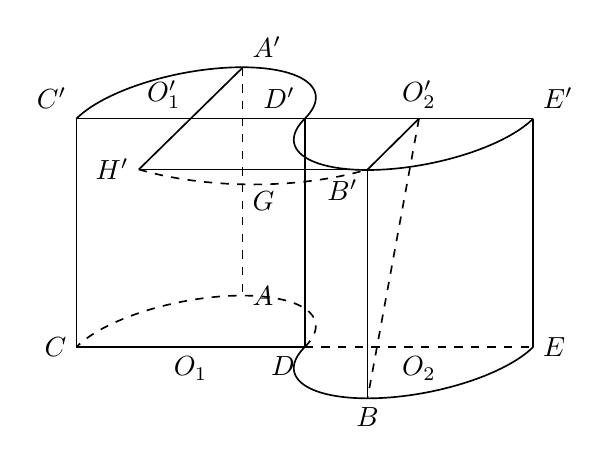
\begin{tikzpicture}[scale=1.45, >=stealth, semithick]
  % 半圆（斜二测投影后的椭圆弧）：左半上、下两弧向左上鼓出，右半两弧向右下鼓出
  \draw plot[domain=0:180, samples=90, smooth]
    ({1+cos(\x)+0.45*sin(\x)}, {2+0.45*sin(\x)});      % 左半顶面，过 A'
  \draw[dashed] plot[domain=0:180, samples=90, smooth]
    ({1+cos(\x)+0.45*sin(\x)}, {0.45*sin(\x)});        % 左半底面，不可见，过 A
  \draw plot[domain=0:180, samples=90, smooth]
    ({3+cos(\x)-0.45*sin(\x)}, {2-0.45*sin(\x)});      % 右半顶面，过 B'
  \draw plot[domain=0:180, samples=90, smooth]
    ({3+cos(\x)-0.45*sin(\x)}, {-0.45*sin(\x)});       % 右半底面，过 B
  % 切面边与可见棱
  \draw (0,2) -- (0,0) -- (2,0);                        % C'C、CD
  \draw (0,2) -- (4,2);                                 % C'D'E'
  \draw (2,2) -- (2,0);                                 % D'D
  \draw (4,2) -- (4,0);                                 % E'E
  \draw (2.55,1.5545) -- (2.55,-0.4455);                % B'B
  % 左半顶面上的半径 A'O1' 及其延长到 H'
  \draw (1.454,2.4455) -- (0.546,1.5545);               % A'H'，过 O1'(1,2)
  % 右半顶面上的半径 O2'B' 可见，O2'B 藏在体内
  \draw (3,2) -- (2.55,1.5545);                         % O2'B'
  \draw[dashed] (3,2) -- (2.55,-0.4455);                % O2'B
  % AA'（含中点 G）不可见；DE 不可见
  \draw[dashed] (1.454,2.4455) -- (1.454,0.4455);       % A'A，过 G(1.454,1.4455)
  \draw[dashed] (2,0) -- (4,0);                         % DE
  % H'B' 实线；其下的微凹虚线弧照原页保留
  \draw (0.546,1.5545) -- (2.55,1.5545);
  \draw[dashed] (0.546,1.5545) .. controls (1.15,1.38) and (1.95,1.38) .. (2.55,1.5545);
  % 顶点与中点标注
  \node[above left]  at (0,2)   {$C'$};
  \node[left]        at (0,0)   {$C$};
  \node[above left]  at (2,2)   {$D'$};
  \node[below left]  at (2,0)   {$D$};
  \node[above right] at (4,2)   {$E'$};
  \node[right]       at (4,0)   {$E$};
  \node[above right] at (1.454,2.4455) {$A'$};
  \node[right]       at (1.454,0.4455) {$A$};
  \node[below left]  at (2.55,1.5545)  {$B'$};
  \node[below]       at (2.55,-0.4455) {$B$};
  \node[left]        at (0.546,1.5545) {$H'$};
  \node[below right] at (1.454,1.4455) {$G$};
  \node[below]       at (1,0)   {$O_1$};
  \node[above left]  at (1,2)   {$O_1'$};
  \node[below]       at (3,0)   {$O_2$};
  \node[above]       at (3,2)   {$O_2'$};
\end{tikzpicture}
